\documentclass[14pt]{beamer}
\usefonttheme[onlymath]{serif}
\usepackage[normalem]{ulem}
\usepackage[T2A]{fontenc}
\usepackage[utf8]{inputenc}
\usepackage[english,russian]{babel}
\usepackage{amssymb,amsfonts,amsmath,mathtext}
\usepackage{cite,enumerate,float,indentfirst}
\usepackage{bm}

\graphicspath{{images/}}

\usetheme{Pittsburgh}
\usecolortheme{whale}

\setbeamercolor{footline}{fg=blue}
\setbeamertemplate{footline}{
  \leavevmode%
  \hbox{%
  \begin{beamercolorbox}[wd=.333333\paperwidth,ht=2.25ex,dp=1ex,center]{}%
    Павлович В. В. | selatnick@gmail.com
  \end{beamercolorbox}%
  \begin{beamercolorbox}[wd=.333333\paperwidth,ht=2.25ex,dp=1ex,center]{}%
    Минск, 2017
  \end{beamercolorbox}%
  \begin{beamercolorbox}[wd=.333333\paperwidth,ht=2.25ex,dp=1ex,right]{}%
  Стр. \insertframenumber{} из \inserttotalframenumber \hspace*{2ex}
  \end{beamercolorbox}}%
  \vskip0pt%
}

\newcommand{\itemi}{\item[\checkmark]}

\title{SVM}
\author{\small{%
\emph{Выступающий:}~Павлович Владислав}
\vspace{20pt}%
}
\date{\small{Минск, 2017}}

\begin{document}
\maketitle

\begin{frame}
\frametitle{Бинарная классификация}
\center{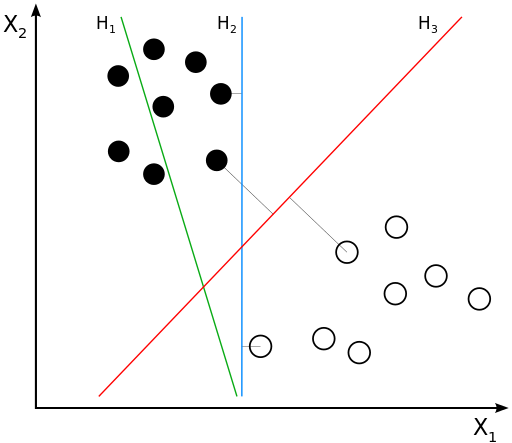
\includegraphics[width=0.6\linewidth]{svm1.png}}
\end{frame}

\begin{frame}
\frametitle{Бинарная классификация}
\begin{itemize}
\item<1-> $\left\{x_i, y_i\right\}, i = 1, \ldots \ell,
    x_i \in \mathbb{R}^D, y_i \in \left\{-1, 1\right\}$.
\item<2-> Выборка линейно разделима.
\item<3-> Будем строить разделяющуя гиперплоскость: $w \cdot x + b = 0$.
  \begin{itemize}
    \item $w$ - вектор нормали.
    \item $\dfrac{b}{||w||}$ - расстояние до начала координат.
  \end{itemize}
\end{itemize}
\end{frame}

\begin{frame}
\frametitle{Бинарная классификация}
\center{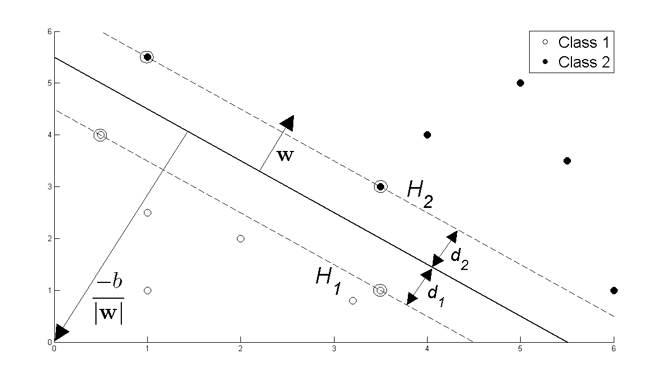
\includegraphics[width=0.8\linewidth]{svm2.png}}
\end{frame}

\begin{frame}
\frametitle{Бинарная классификация}
\begin{align*}
  &\begin{cases}
    &w \cdot x_i + b \geqslant 1, y_i = 1\\
    &w \cdot x_i + b \leqslant -1, y_i = -1
  \end{cases}\Rightarrow\\
  &\Rightarrow y_i (w \cdot x_i + b) \geqslant 1, i = 1, \ldots, \ell.
\end{align*}
\end{frame}

\begin{frame}
\frametitle{Бинарная классификация}
$H_1, H_2$ - множества опорных векторов соответствующих классов.
\begin{align*}
  &\begin{cases}
    &w \cdot x_i + b = 1, i \in H_1\\
    &w \cdot x_i + b = -1, i \in H_2
  \end{cases}
\end{align*}

$d_1, d_2$ - расстояния между гиперплоскостью и опорными векторами.

\begin{align*}
  d_1 = d_2 = \dfrac{1}{||w||}
\end{align*}
\end{frame}

\begin{frame}
\frametitle{Бинарная классификация}
\begin{itemize}
  \item<1-> $\min ||w|| \text{ т.ч. } y_i(x_i \cdot w + b) - 1 \geqslant 0, \forall i = 1, \ldots \ell$.
  \item<2-> $\min \dfrac{1}{2}||w||^2 \text{ т.ч. } y_i(x_i \cdot w + b) - 1
             \geqslant 0$, ${\forall i = 1, \ldots \ell}$ - задача
            квадратичного программирования.
\end{itemize}
\end{frame}

\begin{frame}
\frametitle{Бинарная классификация}
Метод множителей Лагранжа
\begin{itemize}
  \item<1-> $L_P = \dfrac{1}{2}||w||^2 - \sum\limits_{i = 1}^{\ell}
      \alpha_iy_i(x_i \cdot w + b) + \sum\limits_{i = 1}^{\ell}\alpha_i$.
  \item<2-> $\dfrac{\partial L_P}{\partial w} = 0 \Rightarrow
      w = \sum\limits_{i = 1}^{\ell}\alpha_iy_ix_i$.
  \item<3-> $\dfrac{\partial L_P}{\partial b} = 0 \Rightarrow
      \sum\limits_{i = 1}^{\ell}\alpha_iy_i = 0$.
\end{itemize}
\end{frame}

\begin{frame}
\frametitle{Бинарная классификация}
\begin{align*}
  &L_D = \sum\limits_{i = 1}^{\ell}\alpha_i - \dfrac{1}{2}
  \sum\limits_{i, j = 1}^{\ell}\alpha_i\alpha_jy_iy_j x_i \cdot x_j,\\
  &\alpha_i \geqslant 0, \forall i = 1, \ldots \ell,
  \sum\limits_{i = 1}^{\ell}\alpha_iy_i = 0.\\
  &L_D = \sum\limits_{i = 1}^{\ell}\alpha_i - \dfrac{1}{2}\alpha^TH\alpha\\
  &\alpha_i \geqslant 0, \forall i = 1, \ldots \ell,
  \sum\limits_{i = 1}^{\ell}\alpha_iy_i = 0.\\
\end{align*}
\end{frame}

\begin{frame}
\frametitle{Бинарная классификация}
Задача квадратичного программирования:
\begin{align*}
  &\underset{\alpha}{\max}\left[\sum\limits_{i = 1}^{\ell}\alpha_i - \dfrac{1}{2}\alpha^TH\alpha\right]\\
  &\alpha_i \geqslant 0, \forall i = 1, \ldots \ell,
   \sum\limits_{i = 1}^{\ell}\alpha_iy_i = 0.\\
\end{align*}

\begin{itemize}
  \item<2-> Находим $\alpha$.
  \item<3-> Вычисляем $w = \sum\limits_{i = 1}^{\ell}\alpha_iy_ix_i$.
\end{itemize}
\end{frame}

\begin{frame}
\frametitle{Бинарная классификация}
\begin{align*}
  &y_s(x_s \cdot w + b) = 1, x_s \text{ - опорный вектор}\\
  &y_s\left(\sum\limits_{m \in S}\alpha_m y_m x_m \cdot x_s + b\right) = 1\\
  &x_i - \text{ опорный вектор, если } \alpha_i > 0.\\
  &y_s^2\left(\sum\limits_{m \in S}\alpha_m y_m x_m \cdot x_s + b\right) = y_s\\
  &b = y_s - \sum\limits_{m \in S}\alpha_m y_m x_m \cdot x_s = y_s - w \cdot x_s\\
  &b = \dfrac{1}{N_S}\sum\limits_{s \in S}\left(y_s - w \cdot x_s \right)
\end{align*}
\end{frame}

\begin{frame}
\frametitle{Бинарная классификация}
\begin{align*}
  y' = \mathtt{sgn}(x \cdot w + b)
\end{align*}
\end{frame}

\begin{frame}
\frametitle{Линейно неразделимые выборки}
\center{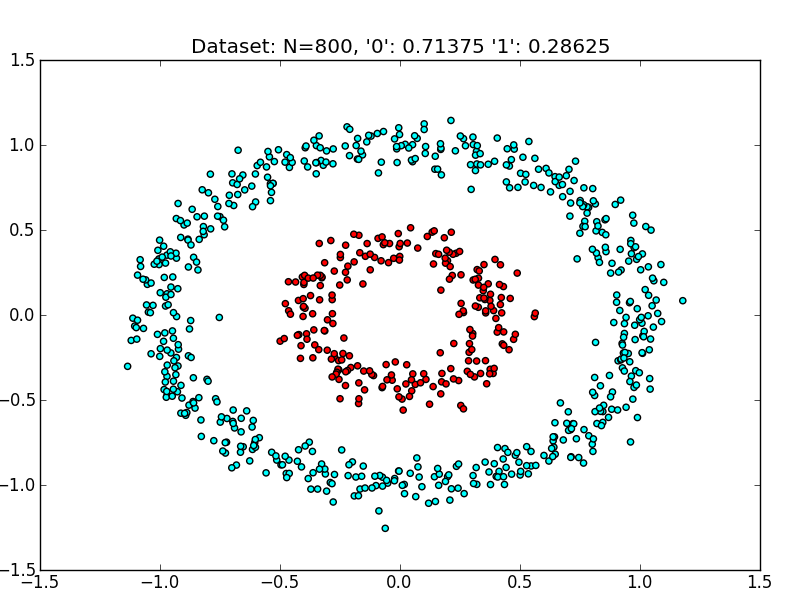
\includegraphics[width=0.8\linewidth]{svm3.png}}
\end{frame}

\begin{frame}
\frametitle{Линейно неразделимые выборки}
Soft margin
\begin{align*}
  &\begin{cases}
    &w \cdot x_i + b \geqslant 1 - \xi_i, y_i = 1\\
    &w \cdot x_i + b \leqslant -1 + \xi_i, y_i = -1
  \end{cases}\Rightarrow\\
  &\Rightarrow y_i (w \cdot x_i + b) - 1 + \xi_i \geqslant 0, \xi_i \geqslant 0,
    i = 1, \ldots, \ell.
\end{align*}
\end{frame}

\begin{frame}
\frametitle{Линейно неразделимые выборки}
\center{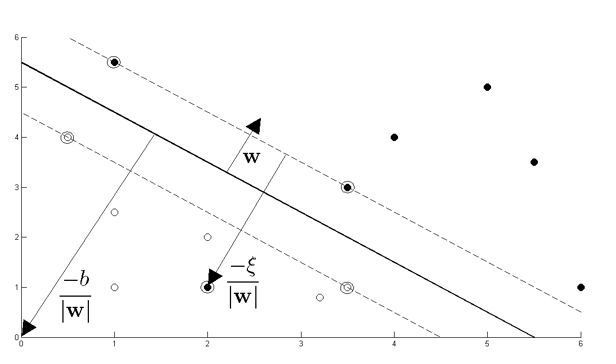
\includegraphics[width=0.8\linewidth]{svm4.png}}
\end{frame}

\begin{frame}
\frametitle{Линейно неразделимые выборки}
\begin{align*}
  &\min \dfrac{1}{2}||w||^2 + C\sum\limits_{i = 1}^{\ell}\xi_i\\
  &\text{ т.ч. } y_i(x_i \cdot w + b) - 1 + \xi_i \geqslant 0, \xi_i \geqslant 0, {\forall i = 1, \ldots \ell}
\end{align*}
\end{frame}

\begin{frame}
\frametitle{Линейно неразделимые выборки}
\begin{itemize}
  \item<1-> ${L_P = \dfrac{1}{2}||w||^2 + C\sum\limits_{i = 1}^{\ell}\xi_i
      - \sum\limits_{i = 1}^{\ell}\mu_i\xi_i} - $
      ${- \sum\limits_{i = 1}^{\ell}\alpha_i[y_i(x_i \cdot w + b) - 1 + \xi_i]}$.
  \item<2-> $\dfrac{\partial L_P}{\partial w} = 0 \Rightarrow
      w = \sum\limits_{i = 1}^{\ell}\alpha_iy_ix_i$.
  \item<3-> $\dfrac{\partial L_P}{\partial b} = 0 \Rightarrow
      \sum\limits_{i = 1}^{\ell}\alpha_iy_i = 0$.
  \item<4-> $\dfrac{\partial L_P}{\partial \xi_i} = 0 \Rightarrow
      C = \mu_i + \alpha_i$.
\end{itemize}
\end{frame}

\begin{frame}
\frametitle{Линейно неразделимые выборки}
\begin{align*}
  &\underset{\alpha}{\max}\left[\sum\limits_{i = 1}^{\ell}\alpha_i - \dfrac{1}{2}\alpha^TH\alpha\right]\\
  &0 \leqslant \alpha_i \leqslant C, \forall i = 1, \ldots \ell,
   \sum\limits_{i = 1}^{\ell}\alpha_iy_i = 0.\\
\end{align*}
\end{frame}

\begin{frame}
\frametitle{Регрессия}
\begin{itemize}
\item<1-> $\left\{x_i, y_i\right\}, i = 1, \ldots \ell,
    x_i \in \mathbb{R}^D, y_i \in \mathbb{R}$.
\item<2-> $y_i = \mathbf{w} \cdot \mathbf{x_i} + b$.
\end{itemize}
\end{frame}

\begin{frame}
\frametitle{Регрессия}
\center{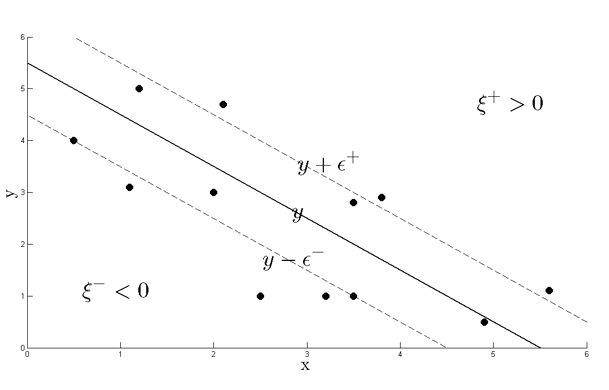
\includegraphics[width=0.8\linewidth]{svm5.png}}
\end{frame}

\begin{frame}
\frametitle{Регрессия}
Интервалы для исходных значений
\begin{align*}
  \begin{cases}
    t_i \leqslant y_i + \varepsilon + \xi^+_i\\
    t_i \geqslant y_i - \varepsilon - \xi^-_i
  \end{cases}
\end{align*}

Функционал ошибки
\begin{align*}
  C\sum\limits_{i = 1}^{\ell}(\xi_i^- + \xi_i^+) + \dfrac{1}{2}||w||^2
\end{align*}
\end{frame}

\begin{frame}
\frametitle{Регрессия}
\begin{align*}
  L_P &= C\sum\limits_{i = 1}^{\ell}(\xi_i^- + \xi_i^+) + \dfrac{1}{2}||w||^2 \\
  &- \sum\limits_{i = 1}^{\ell}(\mu_i^-\xi_i^- + \mu_i^+\xi_i^+)\\
  &- \sum\limits_{i = 1}^{\ell}\alpha_i^+(\varepsilon + \xi_i^+ + y_i - t_i)\\
  &- \sum\limits_{i = 1}^{\ell}\alpha_i^-(\varepsilon + \xi_i^- - y_i + t_i)\\
\end{align*}
\end{frame}

\begin{frame}
\frametitle{Регрессия}
\begin{align*}
  L_P &= C\sum\limits_{i = 1}^{\ell}(\xi_i^- + \xi_i^+) + \dfrac{1}{2}||w||^2 \\
  &- \sum\limits_{i = 1}^{\ell}(\mu_i^-\xi_i^- + \mu_i^+\xi_i^+)\\
  &- \sum\limits_{i = 1}^{\ell}\alpha_i^+(\varepsilon + \xi_i^+ + \mathbf{w}\cdot\mathbf{x_i} + b - t_i)\\
  &- \sum\limits_{i = 1}^{\ell}\alpha_i^-(\varepsilon + \xi_i^- - \mathbf{w}\cdot\mathbf{x_i} - b + t_i)\\
\end{align*}
\end{frame}

\begin{frame}
\frametitle{Регрессия}
\begin{align*}
  &\dfrac{\partial L_P}{\partial \mathbf{w}} = 0 \Rightarrow
  \mathbf{w} = \sum\limits_{i = 1}^{\ell}(\alpha_i^+ - \alpha_i^-)\mathbf{x_i}\\
  &\dfrac{\partial L_P}{\partial b} = 0 \Rightarrow
  \sum\limits_{i = 1}^{\ell}(\alpha_i^+ - \alpha_i^-) = 0\\
  &\dfrac{\partial L_P}{\partial \xi_i^+} = 0 \Rightarrow
  C = \alpha_i^+ + \mu_i^+\\
  &\dfrac{\partial L_P}{\partial \xi_i^-} = 0 \Rightarrow
  C = \alpha_i^- + \mu_i^-
\end{align*}
\end{frame}

\begin{frame}
\frametitle{Регрессия}
\begin{align*}
  L_D &= \sum\limits_{i = 1}^{\ell}(\alpha_i^+ - \alpha_i^-)t_i
   -\varepsilon \sum\limits_{i = 1}^{\ell}(\alpha_i^+ - \alpha_i^-)\\
  &- \dfrac{1}{2}\sum\limits_{i, j = 1}^{\ell}(\alpha_i^+ - \alpha_i^-)(\alpha_j^+ - \alpha_j^-)\mathbf{x}_i \cdot \mathbf{x}_j
\end{align*}
\end{frame}

\begin{frame}
\frametitle{Регрессия}
Задача квадратичного программирования
\begin{align*}
   \underset{\alpha^-, \alpha^+}{\max}\biggl[&\sum\limits_{i = 1}^{\ell}(\alpha_i^+ - \alpha_i^-)t_i
   -\varepsilon \sum\limits_{i = 1}^{\ell}(\alpha_i^+ - \alpha_i^-)\\
   &- \dfrac{1}{2}\sum\limits_{i, j = 1}^{\ell}(\alpha_i^+ - \alpha_i^-)(\alpha_j^+ - \alpha_j^-)\mathbf{x}_i \cdot \mathbf{x}_j\biggr],\\
   &0  \leqslant \alpha_i^-, \alpha_i^+ \leqslant C, \sum\limits_{i = 1}^{\ell}(\alpha_i^+ - \alpha_i^-) = 0.
\end{align*}
\end{frame}

\begin{frame}
\frametitle{Регрессия}
\begin{align*}
  b = \dfrac{1}{N_S}\sum\limits_{s \in S}
    \left(t_i - \varepsilon - \sum\limits_{m = 1}^{\ell}
      (\alpha_i^+ - \alpha_i^-)\mathbf{x}_s \cdot \mathbf{x}_m)\right)
\end{align*}
\end{frame}

\begin{frame}
\frametitle{Регрессия}
\begin{align*}
  y' = \sum\limits_{i = 1}^{\ell}(\alpha_i^+ - \alpha_i^-)\mathbf{x}_i\cdot\mathbf{x} + b
\end{align*}
\end{frame}

\begin{frame}
\frametitle{Kernel trick}
\begin{align*}
  \mathbf{H}: H_{ij} = y_iy_jk(\mathbf{x}_i, \mathbf{x}_j) = \mathbf{x}_i \cdot \mathbf{x}_j.
\end{align*}
\begin{itemize}
  \item<2-> $k$ - ядро.
  \item<3-> $\mathbf{K}: K_{ij} = k(\mathbf{x_i}, \mathbf{x_j})$ - положительно
  полуопределённая матрица: $\sum\limits_{i,j}g_iK_{ij}g_j \geqslant 0, \forall g$.
\end{itemize}
\end{frame}

\begin{frame}
\frametitle{Примеры ядер}
\begin{itemize}
  \item Polynomial: $k(\mathbf{x}_1, \mathbf{x}_2) = (1 + \mathbf{x}_1\cdot \mathbf{x}_2)^k$
  \item Sigmoid: $k(\mathbf{x}_1, \mathbf{x}_2) = \tanh(\alpha\mathbf{x}_2\cdot \mathbf{x}_2 + \beta)$
  \item Gaussian RBF: $k(\mathbf{x}_1, \mathbf{x}_2) = e^{-\left(\dfrac{||\mathbf{x}_1 - \mathbf{x}_2||^2}{2\sigma^2}\right)}$
\end{itemize}
\end{frame}

\begin{frame}
\frametitle{Kernel trick}
\center{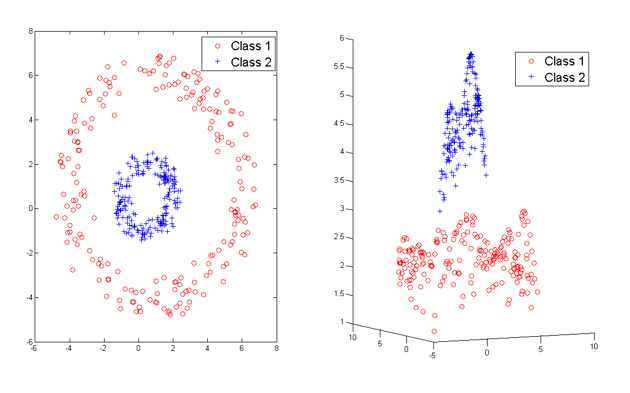
\includegraphics[width=0.8\linewidth]{svm6.png}}
\end{frame}

\end{document}
